%!TEX root = report.tex

Increasingly, gravitational waves are being seen as an exciting method of both testing the predictions of general relativity \cite{lrr-2006-3} and observing effects in astronomy that conventional light based observations would be completely incapable of observing \cite{lrr-2011-1}. We will present two tests of general relativity using gravitational waves.

\section{Gravitational Wave Interferometry}

When we derived the effects of gravitational waves on particles in chapter 3, we saw that gravitational waves had the effect of stretching or compressing an object depending on their polarization and direction compared to the object. A simple test of gravitational waves is therefore to build a device which is sensitive to such changes in its geometry. Such a device is an interferometer.

An interferometer works by producing light of a single wave length from a laser, splitting the light beam into two halves using a beam splitter, sending the beams down two long paths of equal length at 90\(^{\circ}\) to each other and then recombining them. If the beams have been unaffected by their journey they will recombine perfectly. However, if they have not they will form an interference pattern on arrival at the detector.

\begin{figure}[h]
	\centering
	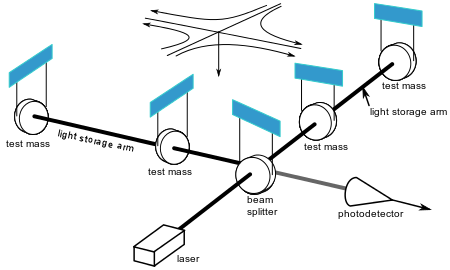
\includegraphics[scale=0.7]{Ligo.png}
	\caption{A diagram of a laser interferometer, adapted from \url{http://www.aei.mpg.de/\~yanbei/page1/page1.html}}
\end{figure}

Currently, such interferometers, such as the Laser Interferometer Gravitational Observatory (LIGO) have not yet seen evidence of gravitational waves, however as the sensitivity increases it is likely they will do so \cite{lrr-2006-3}.

One of the most important future uses of gravitational wave interferometry will be gravitational wave astronomy \cite{lrr-2009-2}, where sources of very strong gravity which cannot be seen using conventional EM radiation astronomy may be observed by gravitational waves.

Unfortunately, as of yet there is no direct evidence for gravitational waves. However, there is indirect evidence for gravitational waves in a strong gravitational situation.

\section{Binary Pulsars}

During a radio survey of pulsars by the Arecibo Radio Telescope in the 1970s a binary system containing two pulsars was discovered. Due to the fast orbit of the two pulsars around each other, gravitational radiation from the orbit slowly carries energy away from the system, decreasing the orbital period.

It is possible to derive an expression for the energy loss due to gravitational radiation by considering the mass moments of the system \cite{cheng}. We will simply state that the rate of energy loss is
\begin{equation} \label{energy-loss}
	\frac{dE}{dt} = \frac{128 G}{5} \omega^6 M^2 R^4
\end{equation}
with \(M\) the mass of the pulsars which are approximately the same, and \(\omega\) the angular frequency. From this equation we can calculate the orbital decay of the system.

If the total energy of the system is \cite{cheng}
\begin{equation} \label{pulsar-energy}
	E = MV^2 = \frac{G M^2}{2R}
\end{equation}
then by considering that \(MV^2 / R = GM^2 / (2R)^2\) we can obtain an equation for \(V^2\)
\begin{equation} \label{v-squared}
	V^2 = \frac{G M}{4R}
\end{equation}
and thus the total energy is
\begin{equation} \label{pulsar-energy2} 
	E = - \frac{G M^2}{4R} .
\end{equation}

If we now rearrange \eqref{v-squared} for \(R\) and note that for an orbit \(V^2 = 2 \pi R / P_{b}\) where \(P_{b}\) is the orbital period then
\begin{equation} \label{radius-pulsar}
	R^3 = \frac{GM}{16 \pi^2} P^2_b
\end{equation}
and thus we can write
\begin{equation} \label{pulsar-energy3}
	E = - M \left( \frac{\pi M G}{2}\right)^{\frac{2}{3}} P_{b}^{- \frac{2}{3}} .
\end{equation}

Now if we rearrange \eqref{pulsar-energy3} for \(P_b\) and differentiate with respect to time we can obtain the rate of orbital period decrease
\begin{equation} \label{orbit-period-decrease}
	\dot{P}_{b} = - \frac{3 P_b}{2 E} \left(\frac{dE}{dt}\right)
\end{equation}
which after substitution of \eqref{pulsar-energy3} and \eqref{energy-loss} becomes
\begin{equation} \label{orbit-period-decrease2}
	\dot{P}_{b} = - \frac{48 \pi}{5} \left( \frac{4 \pi G M}{P_b}\right)^{\frac{5}{3}} .
\end{equation}

By measuring \(P_b\) over time, and examining the results the pulsar's orbital period was seen to be decreasing. The observation of the energy decay over several decades was found to be within 0.3\% accuracy of the result obtained by considering gravitational waves. This is a strong sign that gravitational waves are a phenomenon which do exist.